\documentclass[aps,prx,10pt,twocolumn,floatfix,superscriptaddress,showpacs,numerical,footinbib]{revtex4-1}

\usepackage{graphicx}
\usepackage{amsmath}
\usepackage{amssymb}
\usepackage[utf8]{inputenc}
\usepackage{hyperref}
\usepackage[pdftex]{color}

\newcommand{\sgn}[1]{\mathrm{sgn} \left( #1 \right)}
\newcommand{\e}{\mathrm{e}}
\newcommand{\im}{\mathrm{i}}
\newcommand{\di}{\mathrm{d}}
\newcommand{\ket}[1]{| #1 \rangle}
\newcommand{\bra}[1]{\langle #1 |}
%\renewcommand{\thefootnote}{\fnsymbol{footnote}}

\newcommand{\noteAG}[1]{{\color{blue} [AG: #1]}}
\newcommand{\noteFP}[1]{{\color{magenta} [FP: #1]}}
\newcommand{\noteJM}[1]{{\color{red} [JM: #1]}}
\newcommand{\noteFdJ}[1]{{\color{cyan} [FdJ: #1]}}
\newcommand{\bs}[1]{{\boldsymbol{#1}}}


\begin{document}
%
\title{Interaction driven phases in the half-filled honeycomb lattice: an infinite density matrix renormalization group study}
%
\author{Good people}
\affiliation{\mbox{Max-Planck-Institut f\"ur Physik komplexer Systeme, N\"othnitzer Str.\ 38, 01187 Dresden, Germany}}
%
\date{\today}
%
\begin{abstract}
%
This is an abstract. \noteAG{There are specific commands to leave comments like this one}\noteFP{or this}\noteJM{or this}\noteFdJ{or this}
%
\end{abstract}
%
\maketitle
%

\section{Introduction}
%
The Haldane model~\cite{H88} is amazing.
%
\section{Model and Method}
%
Method\\
%
In this work we focus on spinless electrons in a honeycomb lattice with real  nearest neighbor hopping $t$ and nearest and next to nearest neighbor interactions 
$\left\lbrace V_{1},V_{2}\right\rbrace$. 
%
The Hamiltonian for this system can be written as
 %
\begin{eqnarray}
%
H:=-t\sum_{\left\langle i,j\right\rangle }(c^{\dagger}_{i}c_{j}+h.c.)
%
\;+
V_{1}\sum_{\left\langle i,j\right\rangle }n_{i}n_{j}+
%
V_{2}\sum_{\left\langle \left\langle i,j\right\rangle \right\rangle }n_{i}n_{j}\,
%
\label{eq:H}
%
\end{eqnarray}
%
here $c_{i}$ $(c^{\dagger}_{i})$  annihilates (creates) an electron at the $i$-th site of the honeycomb lattice. 
%
Each of the two triangular sublattices A and B is spanned by the basis vectors
$\bs{a}_{1}=\bs{\delta}_{2}-\bs{\delta}_{3}$ and 
$\bs{a}_{2}=\bs{\delta}_{3}-\bs{\delta}_{1}$ defined through the three nearest neighbors $\bs{\delta}_{1}=a(0,-1)$,  
$\bs{\delta}_{2}=a(\sqrt{3}/2,1/2)$ and $\bs{\delta}_{3}=a(-\sqrt{3}/2,+1/2)$ as shown in Fig.~\ref{fig:Defs}.

\begin{figure}
 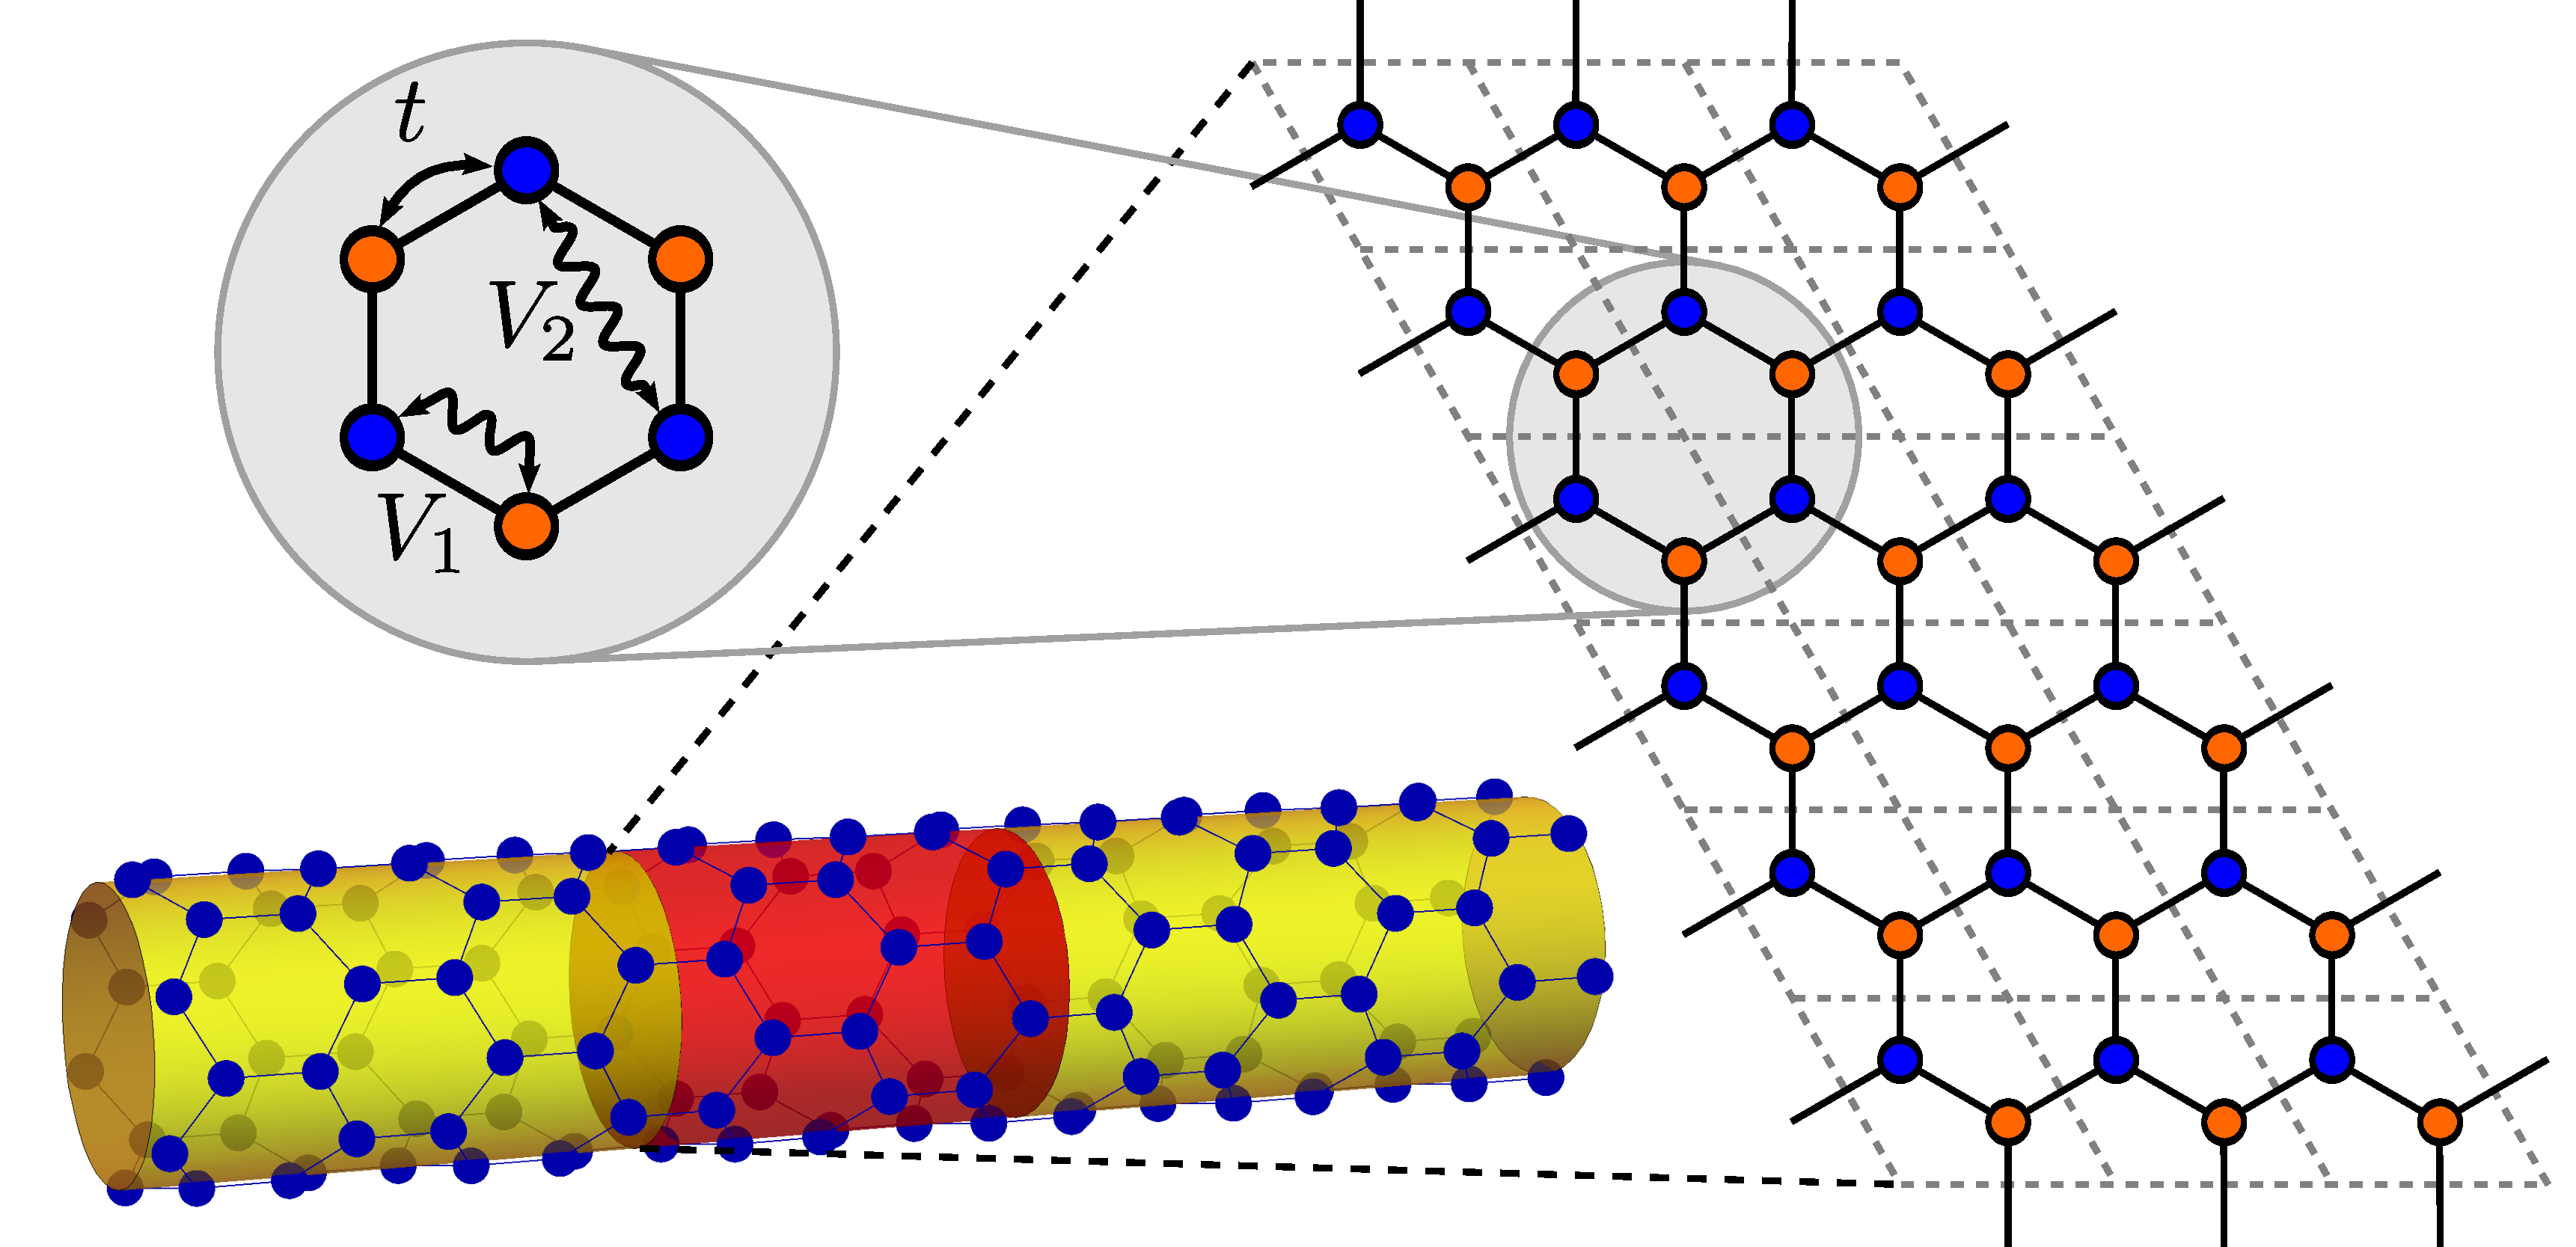
\includegraphics[width=\columnwidth]{pdf/unit_cell.pdf}
 \caption{Unit cell used for the iDMRG calculations. It consists of 3 rings of 12 sites wrapping around the cylinder. The upper and lower edges (green) are connected by periodic boundary conditions. The right and left edges (red) are equivalent. \label{fig:Defs}}
\end{figure}
%
\section{Phase diagram}
%
We have used the iDMRG method presented in the previous section
to find the groundstate of the half-filled graphene lattice 
The main result of this work is the phase diagram presented in Fig.~\ref{fig:phase diagram} obtained
via the iDMRG method.

\begin{figure}
 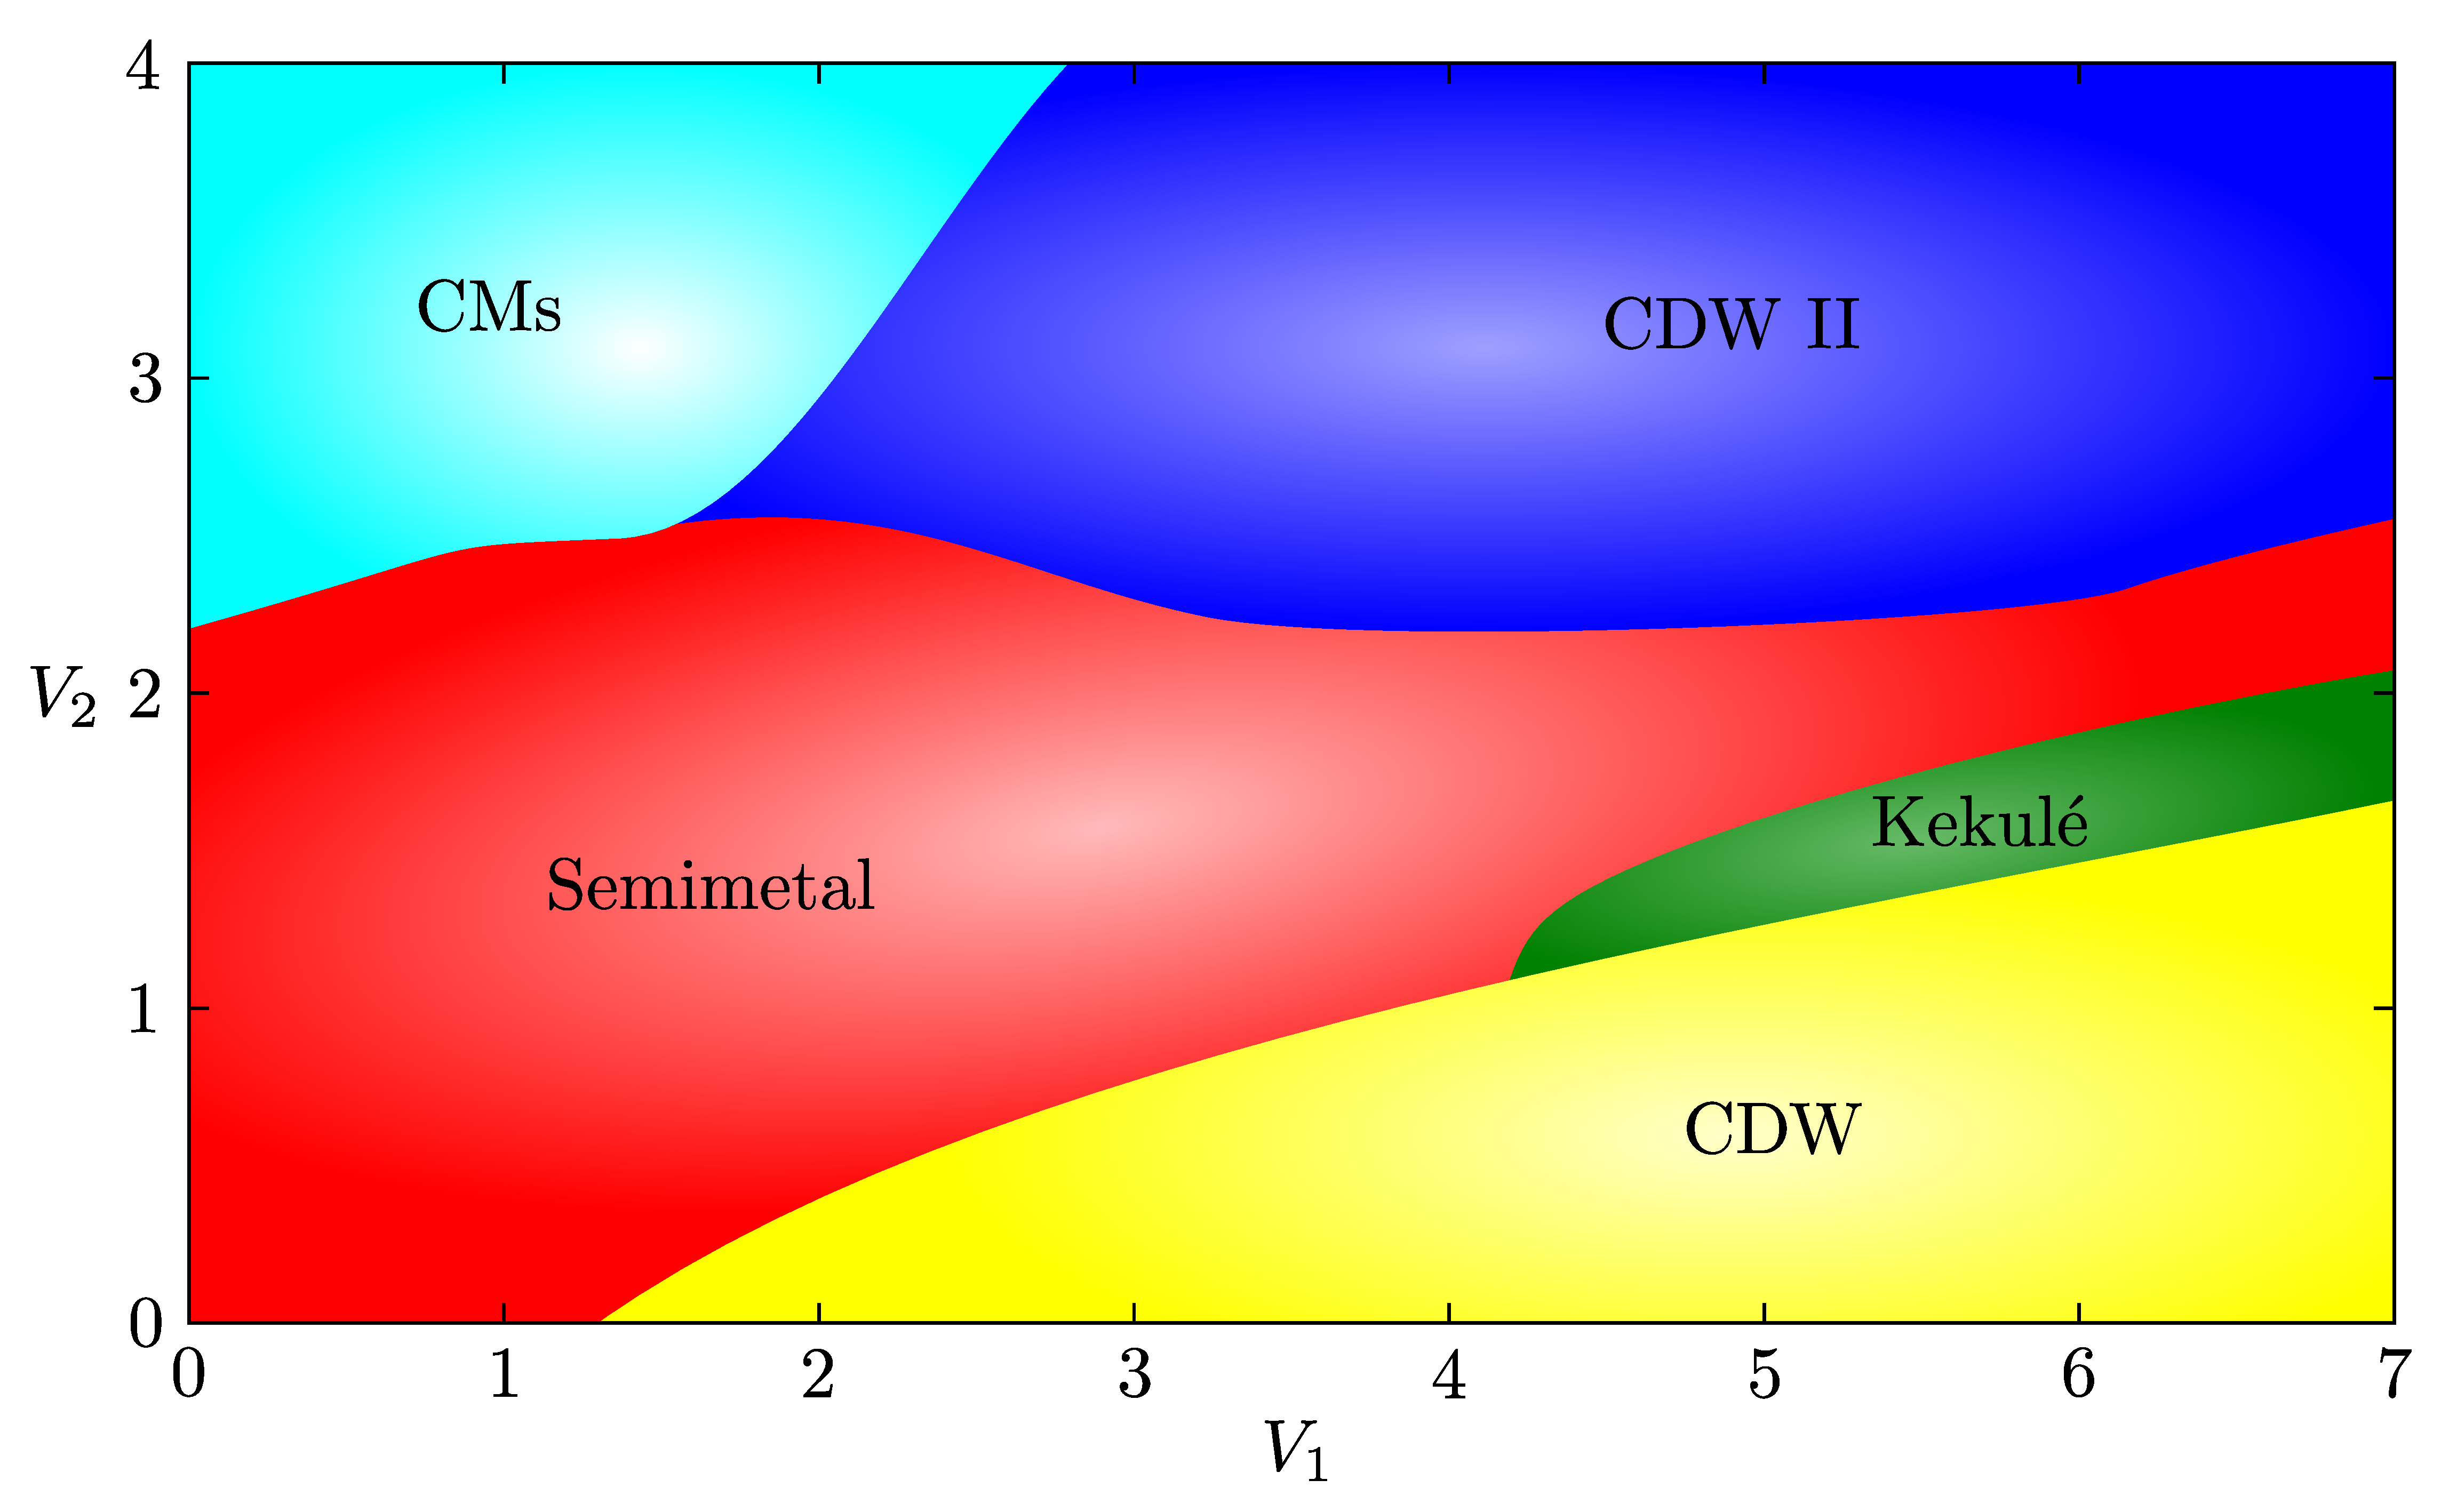
\includegraphics[width=\columnwidth]{pdf/phase_diagram.pdf}
 \caption{Phase diagram obtained with iDMRG calculations on an infinte cylinder of circumference $L=12$. \label{fig:phase diagram}}
\end{figure}

%
\subsection{Semimetal phase}
%
\subsection{Charge density wave}
%
\begin{figure}
 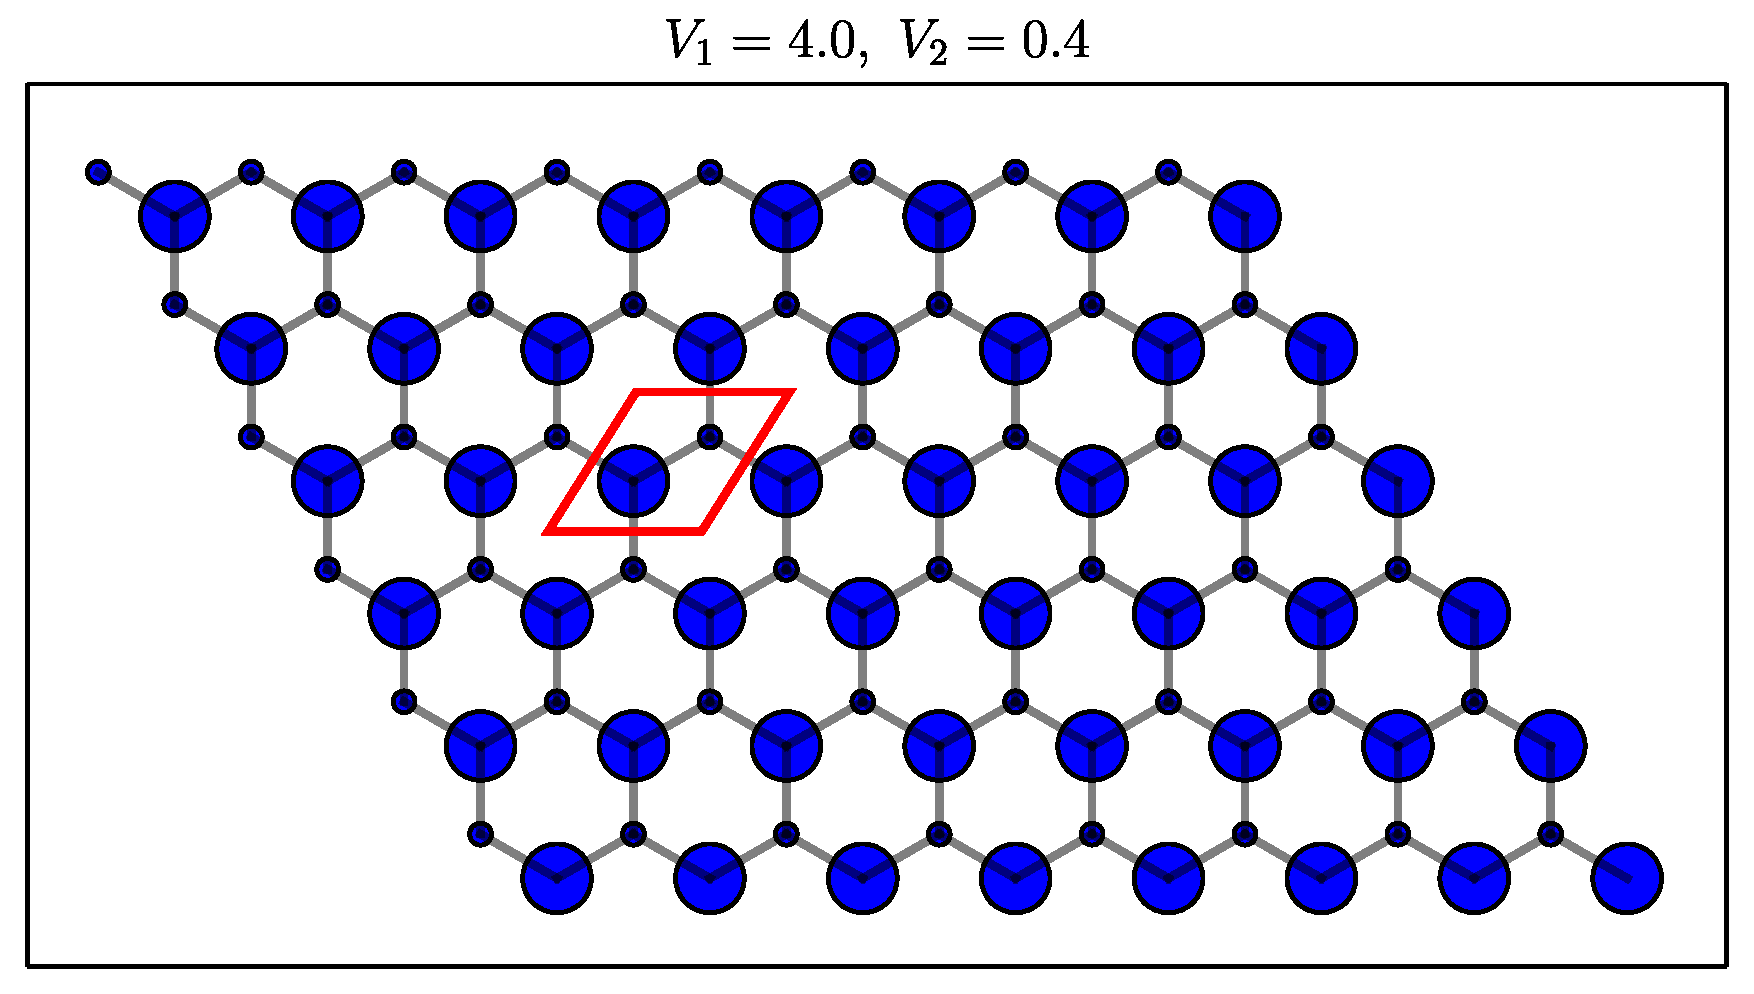
\includegraphics[width=\columnwidth]{pdf/cdw.pdf}
 \caption{Density pattern in the charge density wave phase. The unit cell is depicted by the red rhombus.  \label{fig:cdw}}
\end{figure}

\subsection{Charge modulated phase}
%
\begin{figure}
 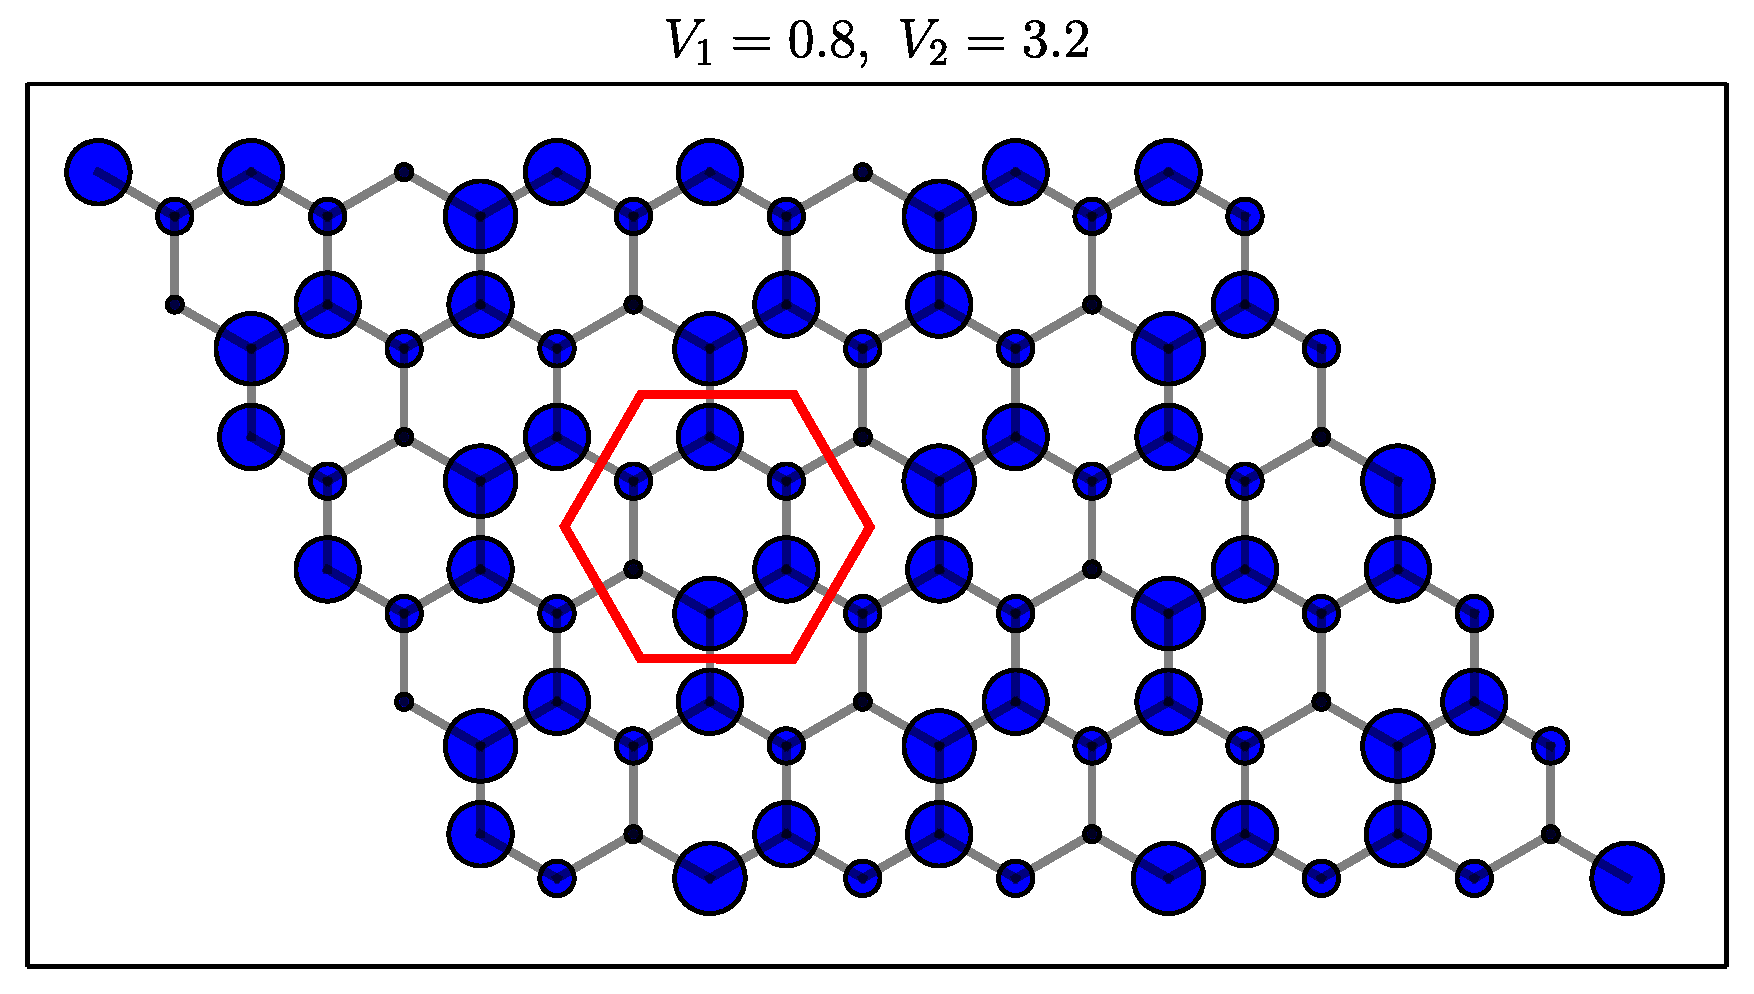
\includegraphics[width=\columnwidth]{pdf/cms.pdf}
 \caption{Density pattern in the charge modulated phase. The unit cell is depicted by the red hexagon.  \label{fig:cms}}
\end{figure}

\subsection{Kekulé}
%
\begin{figure}
 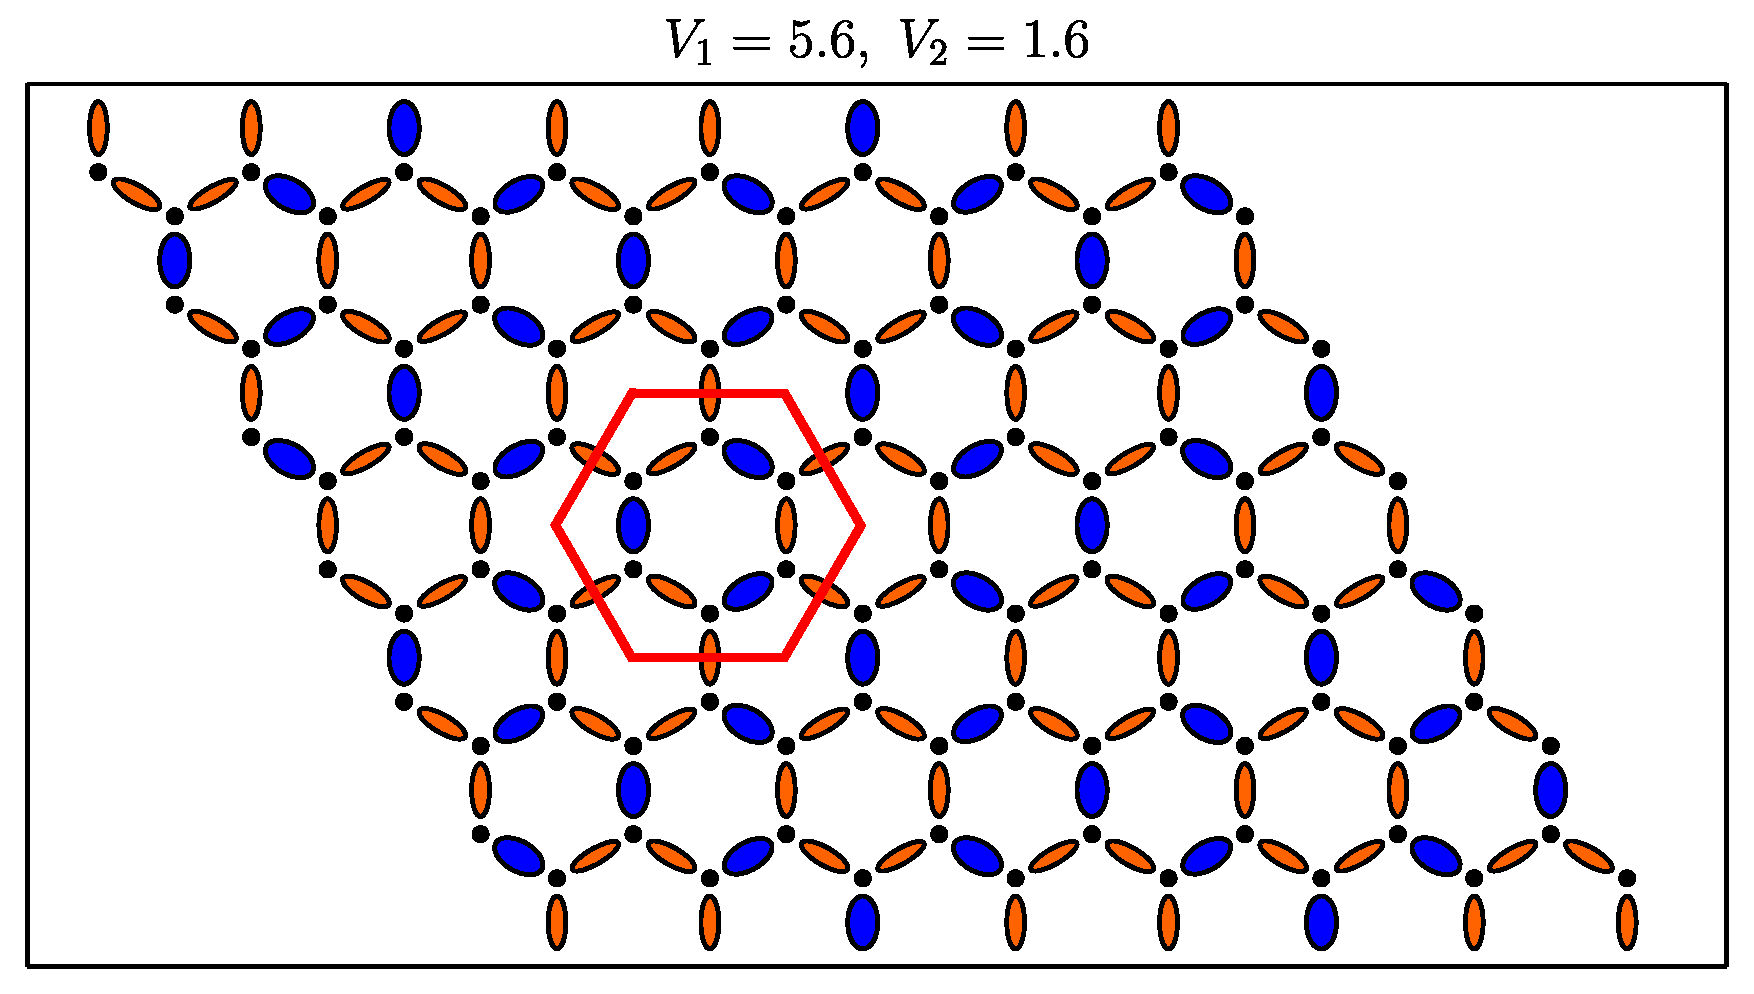
\includegraphics[width=\columnwidth]{pdf/kekule.pdf}
 \caption{Hopping amplitude pattern in the Kekulé phase. The unit cell is depicted by the red hexagon.  \label{fig:kekule}}
\end{figure}

\subsection{Twelve site charge density wave}
%
\begin{figure}
 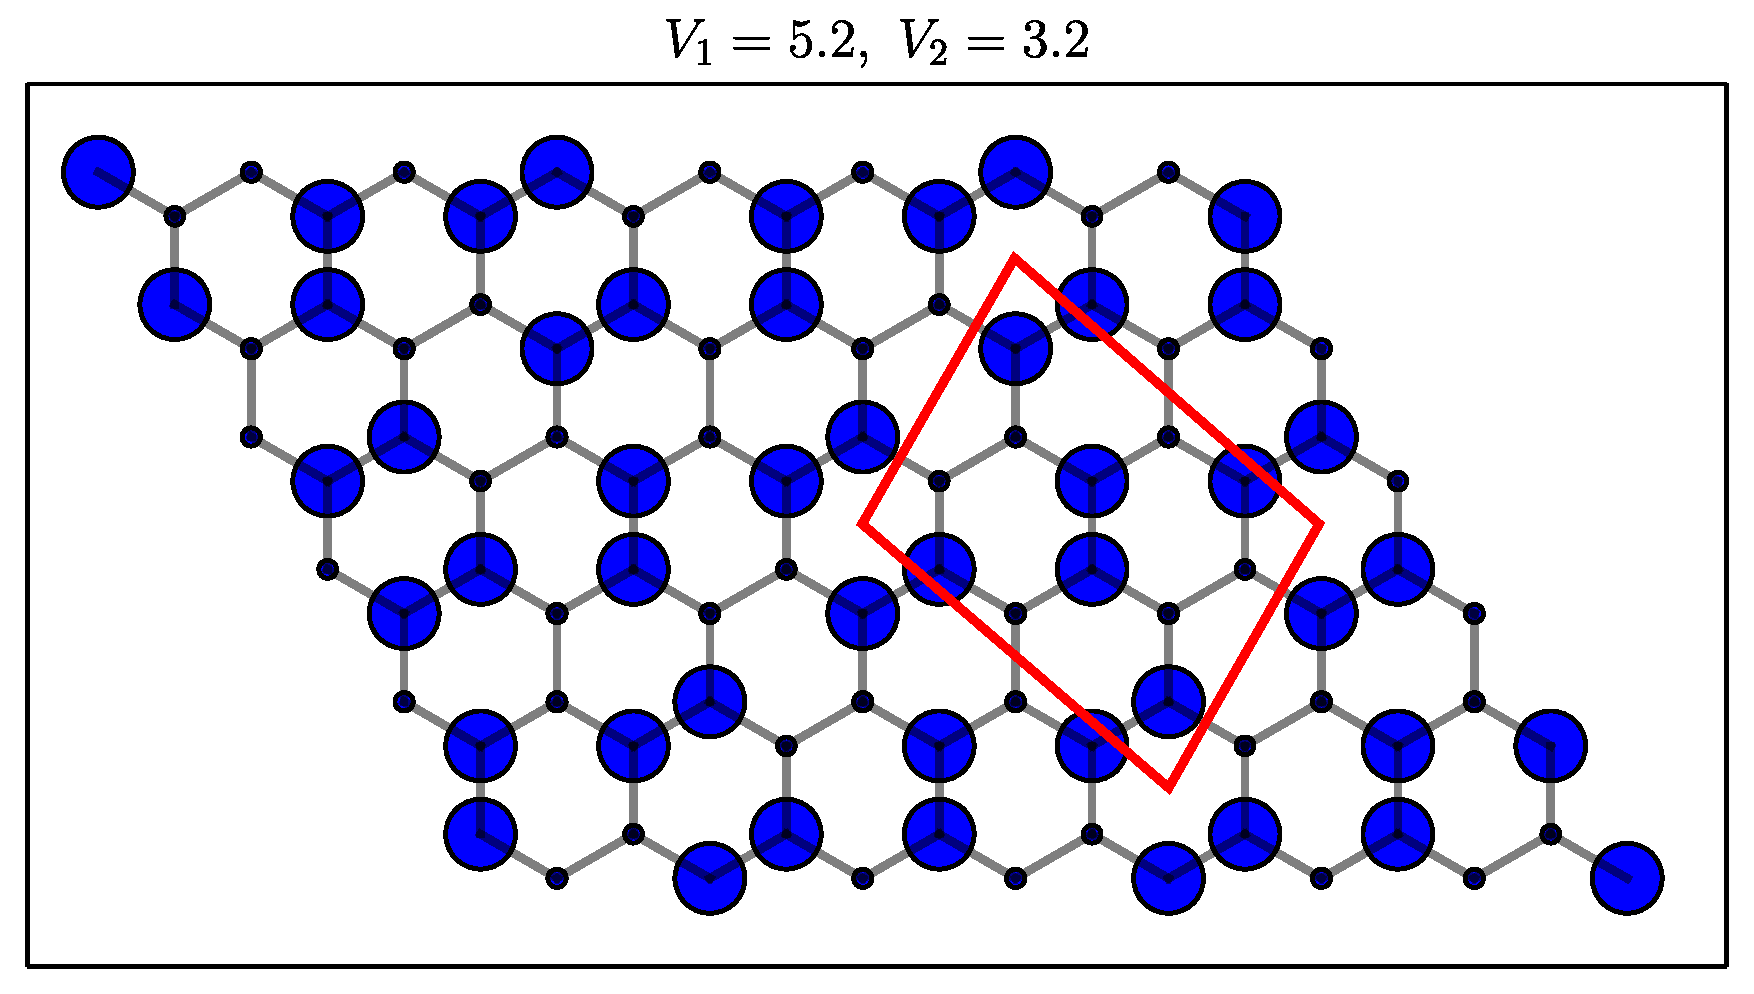
\includegraphics[width=\columnwidth]{pdf/cdw2.pdf}
 \caption{Density pattern in the first twelve site charge density wave phase. The unit cell is depicted by the red rhombus.  \label{fig:cdw2}}
\end{figure}

\subsection{Twelve site charge density wave II}
%
\begin{figure}
 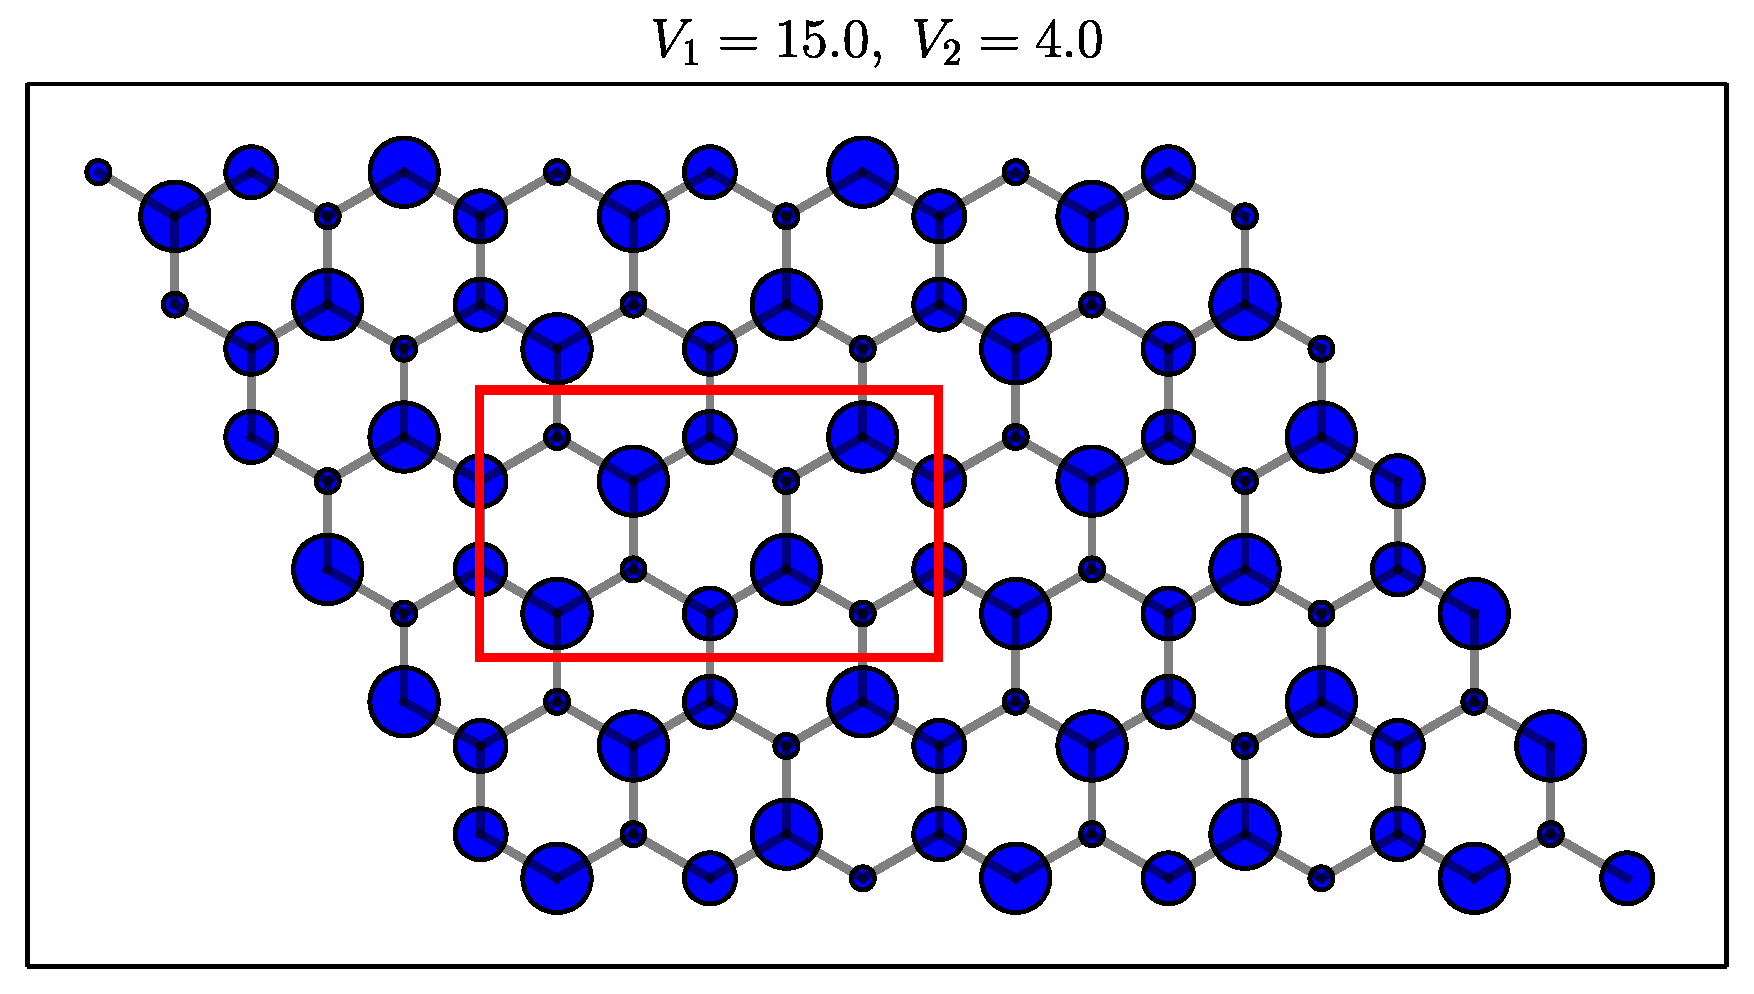
\includegraphics[width=\columnwidth]{pdf/cdw3.pdf}
 \caption{Density pattern in the second twelve site charge density wave phase. The unit cell is depicted by the red rectangle.  \label{fig:cdw3}}
\end{figure}

\section{Phase transitons}
%
some phase transitions?
\begin{figure}
 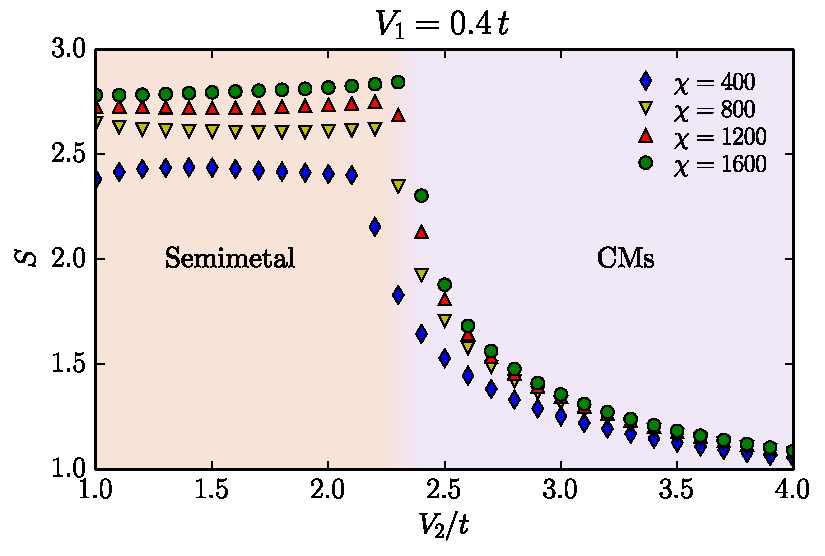
\includegraphics[width=\columnwidth]{{pdf/plot_cut_V1_0.4}.pdf}
 \caption{Entanglement entropy at $V_1=0.4$. \label{fig:cut_V1_0.4}}
\end{figure}

\begin{figure}
 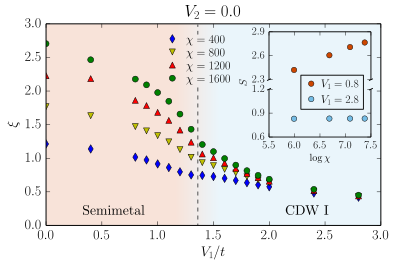
\includegraphics[width=\columnwidth]{{pdf/plot_cut_V2_0}.pdf}
 \caption{Correlation length at $V_2=0$. \label{fig:cut_V2_0}}
\end{figure}

\begin{figure}
 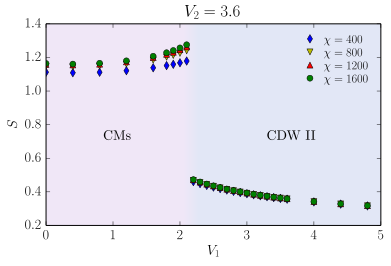
\includegraphics[width=\columnwidth]{{pdf/plot_cut_V2_3.6}.pdf}
 \caption{Entanglement entropy at $V_2=3.6$. \label{fig:cut_V2_3.6}}
\end{figure}

\begin{figure}
 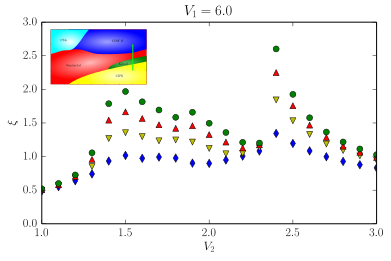
\includegraphics[width=\columnwidth]{{pdf/plot_cut_V1_6}.pdf}
 \caption{Correlation length at $V_1=6$. \label{fig:cut_V1_6}}
\end{figure}



%
\section{Discussion and Conclusions}
%
awesome conclusions

\bibliography{CI_iDMRG.bib}


\end{document}